\documentclass[border=10pt]{standalone}

\usepackage{tikz}
\usepackage{tikzsymbols}
\usetikzlibrary{calc,patterns,shapes.geometric}

\def\centerarc[#1](#2)(#3:#4:#5){\draw[#1] ($(#2)+({#5*cos(#3)},{#5*sin(#3)})$) arc (#3:#4:#5);}

\begin{document}
	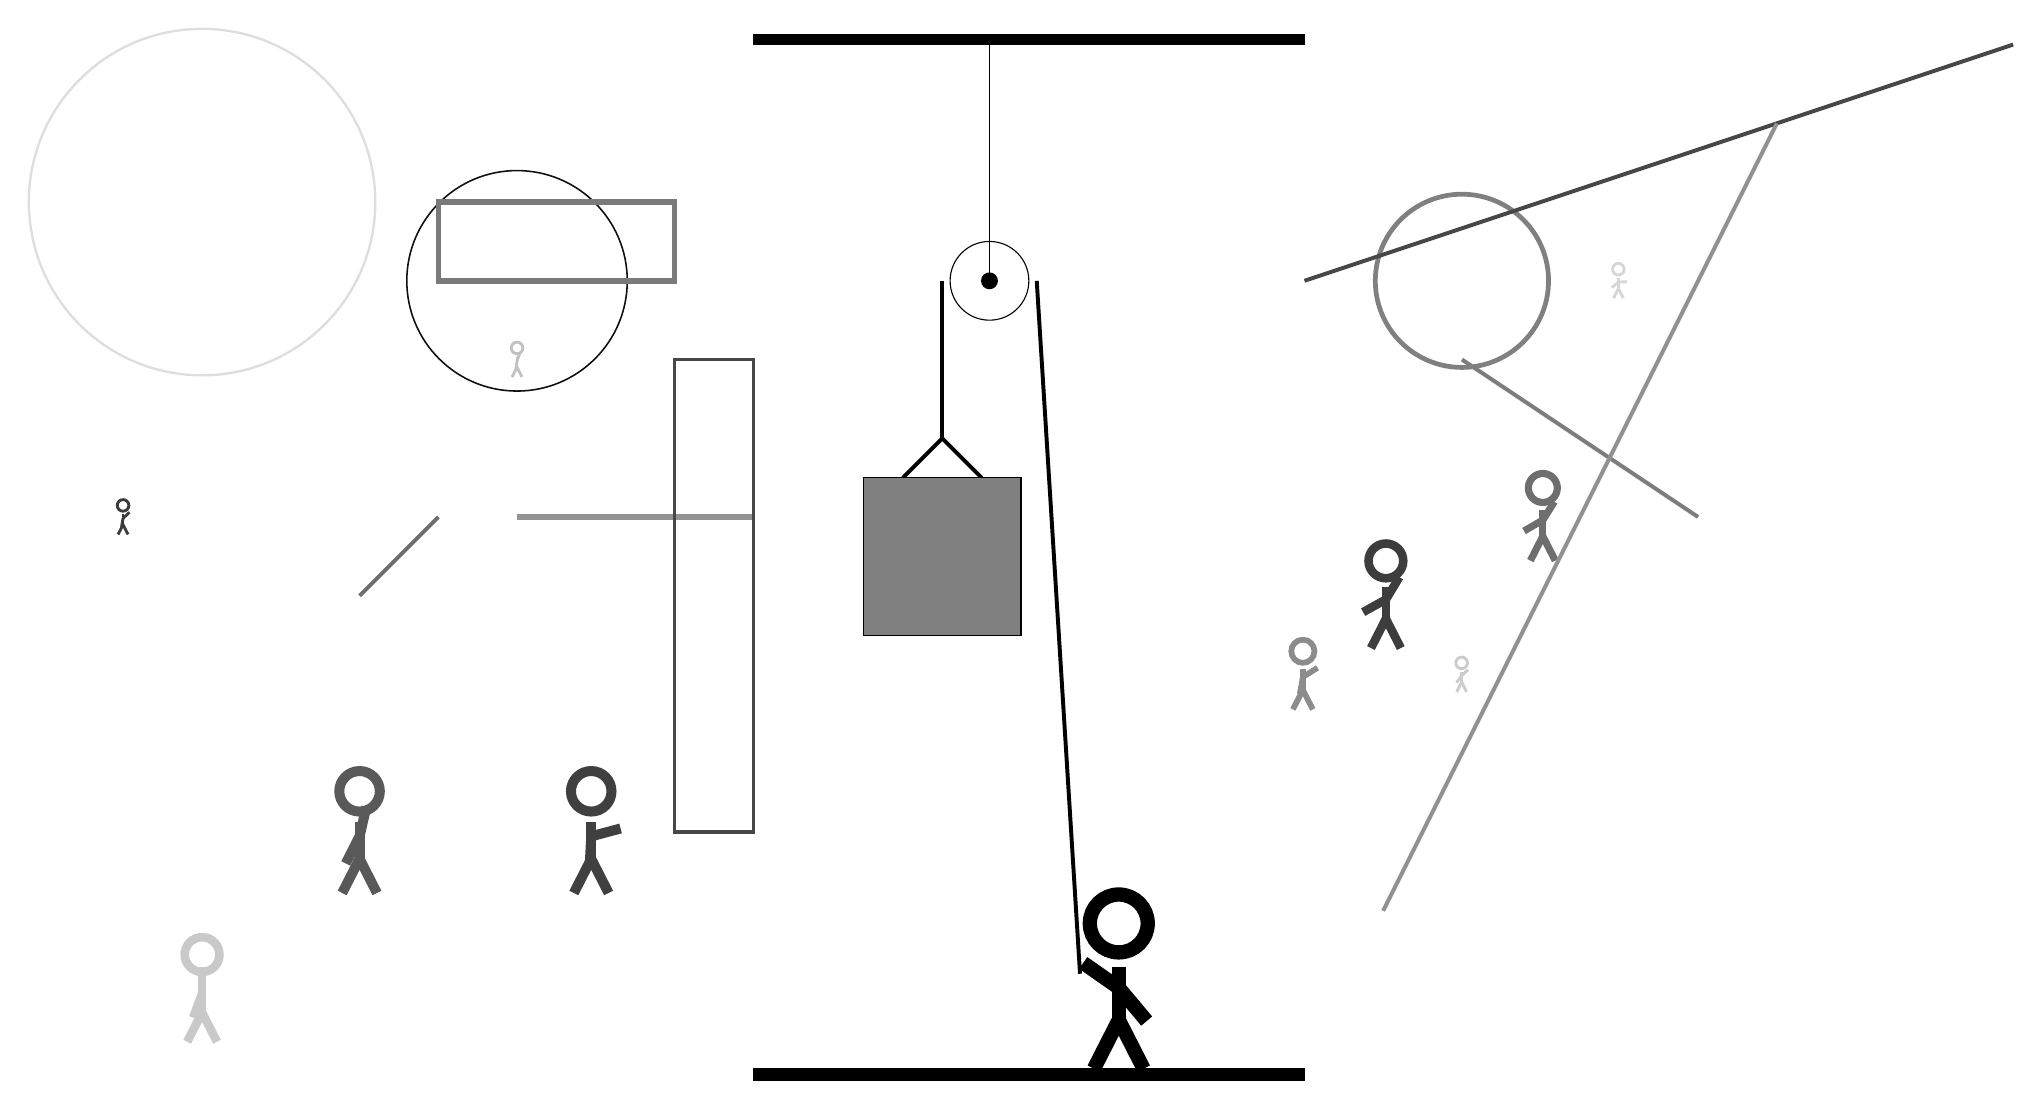
\begin{tikzpicture}
		%%%%% START %%%%%
		
		\draw[fill=black] (-2, 10) rectangle (5, 10.125);
		
		\draw (1, 7) circle (0.5);
		\draw[fill=black] (1, 7) circle (0.1);
		\draw (1, 10) -- (1, 7);
		
		\draw[line width=0.5mm] (-0.1, 4.5) -- (0.4, 5.0) -- (0.9, 4.5);
		\draw[fill=black!50] (-0.6, 4.5) rectangle (1.4, 2.5);
		
		\draw[line width=0.5mm] (0.4, 7) -- (0.4, 5.0);
		\centerarc[line width=0.5mm](1, 7)(0:180:0.6);
		\draw[line width=0.5mm](1.6, 7) -- (2.15, -1.8);
		
		\draw[line width=0.5mm, color=black!57](-6, 4) -- (-7, 3);
		
		\draw [line width=0.2mm, color=black!43](-8, 1) circle (0.0);
		\node[line width=0.6mm, color=black!16] at (9, 7) {\Strichmaxerl[2][40][2]};
		\draw[line width=0.5mm, color=black!51](10, 4) -- (7, 6);
		\node[line width=0.4mm, color=black!57] at (8, 4) {\Strichmaxerl[5][30][58]};
		
		\draw [line width=0.6mm, color=black!50](7, 7) circle (1.1);
		
		\node[line width=0.5mm, color=black!20] at (7, 2) {\Strichmaxerl[2][53][43]};
		\node[line width=0.4mm, color=black!65] at (-7, 0) {\Strichmaxerl[7][63][77]};
		\draw [line width=0.2mm, color=black!94](-5, 7) circle (1.4);
		
		\draw[line width=0.7mm, color=black!52] (-3, 8) rectangle (-6, 7);
		\draw[line width=0.7mm, color=black!42] (-2, 4) rectangle (-5, 4);
		
		\node[line width=0.3mm, color=black!75] at (-4, 0) {\Strichmaxerl[7][87][15]};
		\node[line width=0.3mm, color=black!77] at (-10, 4) {\Strichmaxerl[2][80][43]};
		\node[line width=0.7mm, color=black!45] at (5, 2) {\Strichmaxerl[4][80][32]};
		\draw[line width=0.5mm, color=black!72](5, 7) -- (14, 10);
		\node[line width=0.7mm, color=black!76] at (6, 3) {\Strichmaxerl[6][29][59]};
		\draw [line width=0.3mm, color=black!13](-9, 8) circle (2.2);
		\draw[line width=0.4mm, color=black!72] (-3, 0) rectangle (-2, 6);
		\node[line width=0.5mm, color=black!21] at (-9, -2) {\Strichmaxerl[6][70][90]};
		\draw[line width=0.5mm, color=black!43](6, -1) -- (11, 9);
		\node[line width=0.5mm, color=black!24] at (-5, 6) {\Strichmaxerl[2][83][70]};
		
		
		\node at (2.6, -1.9) {\Strichmaxerl[10][-35][-50]};
		
		\draw[fill=black] (-2, -3) rectangle (5, -3.15);
		
		%%%%% END %%%%%
	\end{tikzpicture}
\end{document}